
\begin{frame}{‌جستجوی عمق‌اول}
\begin{itemize}\itemr
\item[-]
جستجوی عمق‌اول به جای اینکه جستجو را در سطح شروع کند و همهٔ رئوس مجاور را در ابتدا پیمایش کند، به ازای هر رأس پیمایش شده، مجاور رأس را پیمایش می‌کند و به عبارت دیگر جستجو در عمق انجام می‌دهد.
\item[-]
برای روشن‌تر شدن جستجوی سطحی و عمقی مثال زیر را در نظر بگیرید. می‌خواهیم مطلبی را درون چندین کتاب جستجو کنیم. در یک جستجوی سطحی ابتدا به سراغ صفحه اول همهٔ کتاب‌ها می‌رویم تا این که در نهایت همهٔ کتاب‌ها را بررسی کنیم. در یک جستجوی عمقی ابتدا کتاب اول را تا انتها مطالعه می‌کنیم و در صورتی که مطلب مورد نظر را پیدا نکردیم به سراغ کتاب دوم می‌رویم تا این که در نهایت همهٔ کتاب‌ها را جستجو کنیم. در این مثال هیچ یک از جستجوها مزیتی بر دیگری ندارد چرا که مطلب مورد نظر ممکن است در صفحهٔ آخر کتاب اول باشد که در این صورت جستجوی عمقی زودتر به جواب می‌رسد و یا ممکن است مطلب مورد نظر در صفحه اول کتاب آخر باشد که در این صورت جستجوی سطح اول زودتر به جواب می‌رسد.
\end{itemize}
\end{frame}


\begin{frame}{‌جستجوی عمق‌اول}
\begin{itemize}\itemr
\item[-]
جستجوی عمق‌اول یال‌های بررسی نشدهٔ رئوس تازه پیدا شده را زودتر از یال‌های بررسی نشدهٔ رئوس قبلاً پیدا شده بررسی می‌کند. وقتی فرایند جستجو به نقطه‌ای رسید که یال‌های یک رأس همگی بررسی شده بودند، الگوریتم پسگرد می‌کند تا به رئوسی برسد که یال‌های آنها هنوز بررسی نشده‌اند.
\item[-]
در صورتی که یک رأس با شروع از رأس آغازین قابل دسترس نباشد، گراف همبند نیست و برای جستجوی کامل گراف، الگوریتم یکی از رئوس را به عنوان مبدأ جدید انتخاب کرده و جستجو را از رأس جدید آغاز می‌‌کند.
\end{itemize}
\end{frame}


\begin{frame}{‌جستجوی عمق‌اول}
\begin{itemize}\itemr
\item[-]
همانند جستجوی سطح اول، در جستجوی عمق‌اول توسط رنگ رأس‌ها وضعیت آنها مشخص می‌شود. هر رأس در ابتدا سفید است، هنگامی که برای اولین بار پیدا می‌شود به رنگ خاکستری تبدیل می‌شود و در پایان هنگامی که بررسی شد (بدین معنی که همهٔ رئوس در لیست مجاورت آن پیدا شدند) به رنگ سیاه در می‌آید.
\end{itemize}
\end{frame}


\begin{frame}{‌جستجوی عمق‌اول}
\begin{itemize}\itemr
\item[-]
در جستجوی عمق‌اول هر رأس دارای دو برچسب زمان
\fn{1}{time stamp}
است. برچسب زمان اول
\m{v.s}
زمانی نشان می‌دهد که رأس برای بار اول پیدا شده است و به رنگ خاکستری درآمده است و برچسب دوم
\m{v.f}
مشخص می‌کند که رأس
\m{v}
به طور کامل بررسی شده است بدین معنی که همهٔ رئوس لیست مجاورت آن پیدا شده‌اند و رأس
\m{v}
به رنگ مشکی درآمده است.
\end{itemize}
\end{frame}


\begin{frame}{‌جستجوی عمق‌اول}
\begin{itemize}\itemr
\item[-]
الگوریتم زیر جستجوی عمق‌اول را نشان می‌دهد.
\begin{algorithm}[H]\alglr
  \caption{Depth-First Search} 
  \begin{algorithmic}[1]
   \Func{DFS}{G}
   \For{each vertex u $\in$ G.V}
   			\State u.color = White
   			\State u.pred = Nil
   	\EndFor
   	\State time = 0
   	\For{each vertex u $\in$ G.V}
   			\If{u.color == White}
   					\State DFS-Visit(G,u)
   			\EndIf
   	\EndFor                           
  \end{algorithmic}
  \label{alg:merge}
\end{algorithm}
\end{itemize}
\end{frame}


\begin{frame}{‌جستجوی عمق‌اول}
\begin{itemize}\itemr
\item[-]
\begin{algorithm}[H]\alglr
  \caption{DFS-Visit} 
  \begin{algorithmic}[1]
   \Func{DFS-Visit}{G,u}
   \State time = time + 1		\LeftComment{white vertex u has just been discovered}
   \State u.s = time
   \State u.color = Gray
   \For{each vertex v in G.Adj[u]}		\LeftComment{explore each edge(u,v)}
   		\If{v.color == White}
   				\State v.pred = u
   				\State DFS-Visit(G,v)
   		\EndIf
   \EndFor
   \State time = time + 1
   \State u.f = time
   \State u.color = Black   \LeftComment{blacken u; it is finished}                           
  \end{algorithmic}
  \label{alg:merge}
\end{algorithm}
\end{itemize}
\end{frame}


\begin{frame}{‌جستجوی عمق‌اول}
\begin{itemize}\itemr
\item[-]
وقتی الگوریتم جستجوی عمق‌اول به اتمام می‌رسد هر رأس دارای دو برچسب زمان است که یکی زمان پیدا شدن
\fn{1}{discovery time}
و دیگری زمان به پایان رسیدن
\fn{2}{finish time}
را نشان می‌دهد.
\end{itemize}
\end{frame}


\begin{frame}{‌جستجوی عمق‌اول}
\begin{itemize}\itemr
\item[-]
در مثال زیر، گراف توسط الگوریتم عمق‌اول بررسی شده است.
\begin{figure}
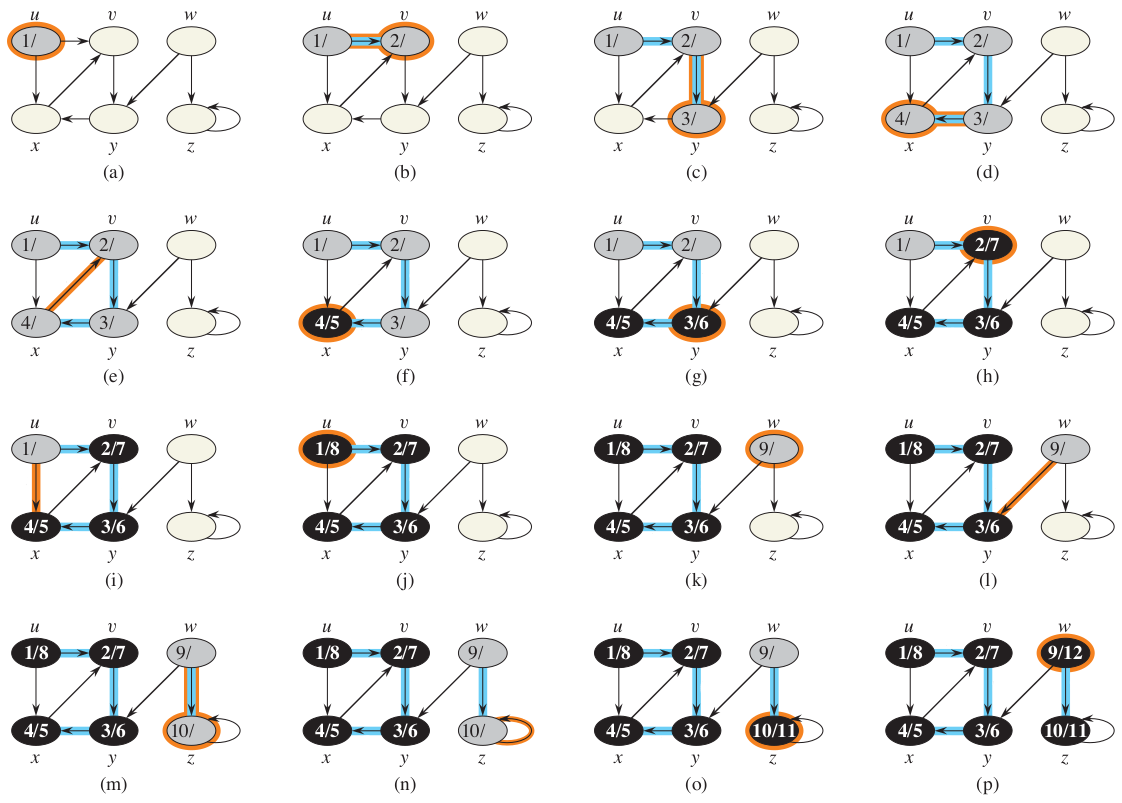
\includegraphics[width=0.6\textwidth]{figs/chap07/566-dfs}
\end{figure}
\end{itemize}
\end{frame}


\begin{frame}{‌جستجوی عمق‌اول}
\begin{itemize}\itemr
%\item[-]
%خطوط ۱ تا ۳ و خطوط ۵ تا ۷ در الگوریتم جستجوی عمق‌اول در زمان
%\ath{V}
%انجام می‌شوند.
\item[-]
در اینجا نیز برای تحلیل الگوریتم از تحلیل تجمعی استفاده می‌کنیم.
\item[-]
الگوریتم
\code{DFS-Visit}
برای هر رأس
\m{v \in V}
تنها یک بار فراخوانی می‌شود، چرا که این الگوریتم برای رئوس سفید فراخوانی می‌شود و آنها را به رنگ خاکستری تبدیل می‌کند. الگوریتم
\code{DFS-Visit}
به ازای هر رأس
\m{v}
در یک حلقه تکرار
\m{|Adj[v]|}
بار تکرار می‌شود. بنابراین برای همهٔ رئوس، این حلقه
\m{\sum_{v \in V} |Adj[v]| = \ath{E}}
بار تکرار می‌شود.
\item[-]
پس زمان اجرای الگوریتم جستجوی عمق‌اول
\ath{V+E}
است.
\end{itemize}
\end{frame}


\begin{frame}{‌جستجوی عمق‌اول}
\begin{itemize}\itemr
\item[-]
می‌توان اثبات کرد که در جستجوی عمق‌اول زمان پیدا شدن و زمان به اتمام رسیدن رئوس گراف یک ساختار پرانتز گذاری کامل دارند. اگر به ازای یافته شدن رأس
\m{u}
یک پرانتز به صورت
\m{"(u"}
باز کنیم و به ازای به اتمام رسیدن بررسی رأس
\m{u}
پرانتز را به صورت
\m{"u)"}
ببندیم، یک عبارت با پرانتزگذاری کامل به دست می‌آید بدین معنی که پرانتزها تودرتو هستند.
\end{itemize}
\end{frame}


\begin{frame}{‌جستجوی عمق‌اول}
\begin{itemize}\itemr
\item[-]
از جستجوی عمق‌اول در مرتب‌سازی توپولوژیکی
\fn{1}{topological sort}
یا مرتب‌سازی موضعی
یک گراف بدون دور
\fn{2}{acyclic graph}
استفاده می‌شود.
\item[-]
یک مرتب‌سازی توپولوژیکی در یک گراف بدون دور
\m{G=(V,E)}
رئوس گراف را به گونه‌ای مرتب می‌کند که اگر
\m{G}
شامل یال
\m{(u,v)}
باشد، آنگاه
\m{u}
قبل از
\m{v}
در آرایهٔ مرتب شده قرار می‌گیرد.
\item[-]
مرتب‌سازی توپولوژیکی تنها برای گراف‌های جهت‌دار بدون دور
\fn{3}{directed acyclic graph}
تعریف می‌شود.
\item[-]
مرتب‌سازی توپولوژیکی به گونه‌ای است که اگر رئوس مرتب شده برروی یک خط افقی قرار بگیرند، جهت همهٔ یال‌های از چپ به راست است.
\end{itemize}
\end{frame}


\begin{frame}{‌جستجوی عمق‌اول}
\begin{itemize}\itemr
\item[-]
از یک گراف جهت‌دار بدون دور می‌توان برای نمایش دادن رویداد‌ها
\fn{1}{event}
استفاده کرد.
\item[-]
برای مثال در شکل زیر برای یک گراف شامل تعدادی رویداد مرتب‌سازی توپولوژیکی انجام شده است.
\begin{figure}
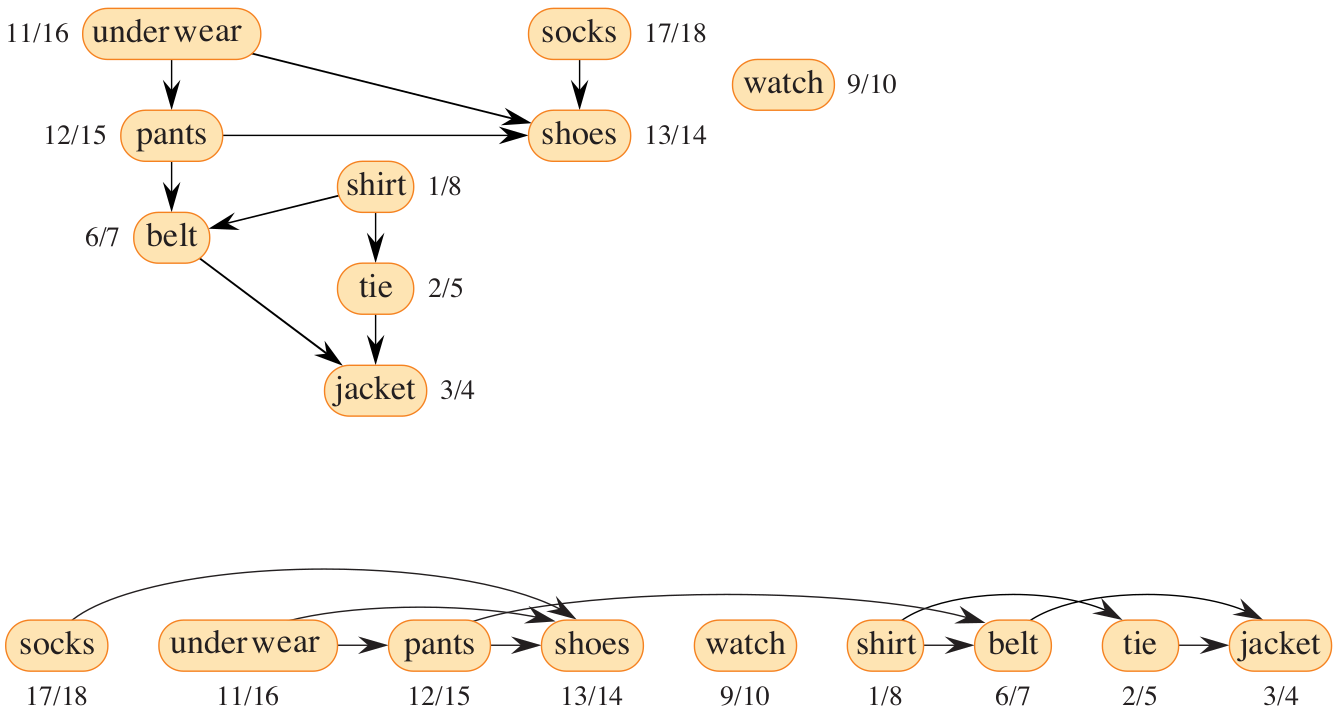
\includegraphics[width=0.6\textwidth]{figs/chap07/574-topological}
\end{figure}
\end{itemize}
\end{frame}